%=== Chapter One ===
\chapter{Combined Literature Review}

%\ifpdf
%    \graphicspath{{Chapter1/Chapter1Figs/PNG/}{Chapter1/Chapter1/PDF/}{Chapter1/Chapter1Figs/}}
%\else
%    \graphicspath{{Chapter1/Chapter1Figs/EPS/}{Chapter1/Chapter1/}}
%\fi

\section{Robotic Path Planning}

\subsection{Introduction}
There has been more than 50 years of progress in robotic path planning, at least a substantial proportion regarding the paths of wheeled mobile robots moving in a two dimensional plane. The goal of this review is not to provide a complete reference, but to justify a certain approach to the problem which is appropriate for the domain of car-like automated vehicles moving goods in automated warehouses.

The central problem is that of a vehicle which follows a defined reference path through a known environment. In some situations the environment may change in such a way that the reference path is no longer feasible. In this case a new path must be generated based on the local information available to the vehicle, and that available from communicating vehicles. This is called Adaptive Local Planning. There are certain requirements for Adaptive Local Planning which are important for the automated warehouse domain more than others. The review reveals that is is more useful to focus on trajectories for the adaptive planning. The trajectories must be feasible in the sense that they meet obstacle avoidance constraints, and in the sense that they meet differential constraints arising from dynamic considerations of the vehicles motion. Furthermore, a guarantee that a path will be found if one exists is a desirable property. It is also desirable for the algorithm to generate a path in a consistent execution time so that the path is always available to the motion control system. In many cases these are conflicting goals: a planner with a hard time limit will not be able to search all possibilities exhaustively. 

\subsection{Planning Architectures}

\cite{Schwarting2018} divide architectures of automated vehicles into three broad categories: Traditional; Behaviour aware, and End-to-end machine learning. Traditional approaches are hierarchical, breaking the problem down into layers including perception, behaviour choice, motion planning, and feedback control. A variety of techniques can then be used at each layer. Perception covers the creation of a representation of the environment from various sensors and lies outside the scope of this review. In the DARPA Urban Challenge contestants this often consisted of a state machine which used expert rules to decide the best manoeuvre such as change lane to be executed by the motion planner \cite{Urmson2008}. The motion planner generated detailed action sequences - trajectories which provide the reference for the feedback control component. 


%\begin{figure}[htbp]
%\begin{center}
%%  \mbox{
%%     \subfigure[]{{\includegraphics[width=0.3\columnwidth, angle=-0]{BehaviourAwareFlowChart}} }
%%     \subfigure[]{{\includegraphics[width=0.3\columnwidth, angle=-0]{BehaviourAwareFlowChart}}}
%%     \subfigure[]{{\includegraphics[width=0.3\columnwidth, angle=-0]{BehaviourAwareFlowChart}}}
%%       }
%\label{fig:broad_categories}
%\end{center}
%\end{figure}

\begin{figure}[ht]
  \begin{center}
	\includegraphics[width=\columnwidth, angle=-0]{HierarchFlowChart}
	\caption{Logical flow of hierarchical planning}
	\label{fig:hierarch_flow}
  \end{center}
\end{figure}
\begin{figure}[ht]
  \begin{center}
	\includegraphics[width=\columnwidth, angle=-0]{EndToEndFlowChart}
	\caption{Logical flow of end-to-end planning}
	\label{fig:endtoend_flow}
  \end{center}
\end{figure}
\begin{figure}[ht]
  \begin{center}
	\includegraphics[width=\columnwidth, angle=-0]{BehaviourAwareFlowChart}
	\caption{Logical flow of interactive behaviour aware planning}
	\label{fig:behaviour_aware_flow}
  \end{center}
\end{figure}

Outcomes can be improved by combining behaviour choice with the motion planner, evaluating different behaviour options to choose the best. For multi-vehicle situations this can lead to interesting behaviour as some model of other vehicles decisions is needed in order to evaluate possible control actions. This could be obtained by inter-vehicle communication or traffic rules based and behavioural models of human traffic participants. At this stage, bringing in multiple participants is also out of scope, but the motion planning component may be useful to inform the type of plans which it is possible to exchange by inter-vehicle communication. Understanding the detail available in a single vehicle's trajectory plan determines the information it can share and also the way it can adapt to the plans of others.

An interesting recent addition to the list of architectures, end-to-end planning \ref{fig:endtoend_flow} eschews traditional distinctions such as perception from planning to instead train an artificial neural network (ANN) on image data from example test drives, so they are able to produce suitable steering commands based on the current video scene in \cite{Chi2017}. To get good results it was necessary to manipulate the training data by creating duplicate runs with a perspective offset, and a larger steering angle to correct the position. Otherwise there were not enough instances of large steering corrections in the data for a basic proportional controller to be learned which steered more vigorously the further it got from the road centre. Given the algorithm used to manipulate the data fully defined the steering behaviour it is hard to see the benefit of using machine learning in this case. It may be more appropriate to use the ANN to provide the behaviour choice and not the closed loop control, similar to \cite{You2019} where the ANN outputs five states - maintain, accelerate, decelerate, turn-left, turn-right, and operates on a simplified model of the traffic detected based on a grid. The actual actuator control - steering angles and acceleration can be completed separately. This should reduce training time by reducing the complexity of the ANN (fewer layers and fewer outputs) and also reducing the amount of noise as the environment representation is quite clean, reducing the chance of over-fitting. ANN based architectures are a useful complement to traditional methods and may be particularly appropriate when predicting the future actions.

Interactive behaviour aware planning is useful to concentrate on because they can utilize component from traditional planning where they are best suited such as feedback control and machine learning techniques where they are most effective, such as in behaviour choice. 

Hierarchical planning techniques are often based on sampling at some resolution from the configuration space, to create a discrete approximation to the problem which can be solved with graph techniques such as Dijkstra. These are able to guarantee resolution completeness, that up to the sampling resolution if a path exists it will be found.     

\section{Cut from JIRS Introduction}   

\subsection{Motivation for Path Adaptation}
Adaptive local path planning is important for the creation of robotic systems which can perform convincingly in variable environments. The particular environment of interest is one of bounded variation: there exists a fixed path which is preferable in most cases, but in certain circumstances it can be invalidated, for example by an obstacle. In this case it may still be possible for the robot to complete its task with a new path avoiding the obstacle, while keeping within a predefined tolerance of the original path to manage predictability. This paper will detail one approach for creating smooth paths for an autonomous vehicle with differential constraints on its motion, and compare two methods for adapting this path in response to an  obstacle detected by on-board sensors.   

\subsection{Paths and Trajectories}
\label{sec:traj_def}
A path is a continuous sequence of configurations. A trajectory is a continuous sequence of configurations each valid at a particular time. A path can always be extracted from a trajectory by discarding the temporal information, but an additional procedure is required to annotate a path with timing information usually based on a choice of speed profile. To ease computation both sequences may be obtained by dividing planning into two scales. 

\subsection{Division Based on Scale}
\label{sec:scale_division}
Large scale trajectory plans cover longer time periods so they can be called strategic plans by an analogy with business plans which cover longer time periods. At the other end of the spectrum small scale trajectory plans take place over shorter time periods so they might be called tactical plans.

Large scale path plans, having no timing information are usually called global plans. This is to distinguish them from local plans which only cover the immediate vicinity around the robot. 

There is no widely accepted scale threshold at which a plan is considered global, as different robots have different size operating domains. As a guide, a planner would be considered global if it is able to find a path between any two valid configurations in the entire domain of operation. A planner would be described as local if there is any limitation on the distance between the start and goal locations over which it can find a path if one exists. 

Global planning algorithms such as Probabilistic Roadmaps, dense random trees all require a local planner component. This component must be sufficient to connect nearby configurations (reach any final configuration) but does not have to account for obstacles. Obstacles are handled at the global layer. The local planner joins two nearby configurations by rejecting links which intersect with obstacles.  

\subsection{Division Based on Execution} 
There is an alternative definition of the local planner which is used by \cite{Walenta2017}, following the manual for ROS (Robot Operating System), a collection of software libraries (middleware) useful for creating robots \cite{rosbook2016}. Here a local planner is one which is able to generate a feasible path between any two adjacent nodes in the roadmap. It works in conjunction with a roadmap planner which efficiently produces large scale plans using Dijkstra or a related graph method. According to \cite{SicilianoKhatib2016} this approach is known Integration Planning, where the global reasoning is provided by a roadmap planner and augmented with a local trajectory planner which accounts for obstacles. This can comprise either a System for Tactical Planning which recomputes at high frequency a path to the target location or a System of Path Deformation which alters the reference path based on sensor data.

This is different from the definition of a local planner in Section \ref{sec:scale_division} where the local planner is an algorithm with limited capabilities, which is utilised by an obstacle avoiding global planner. To create a ROS *local* trajectory planner, an algorithm for global path planning of the type classified in Section \ref{sec:scale_division} would be needed, along with an appropriate speed profile. This is because a core function of the ROS local trajectory planner is obstacle avoidance.


\subsection{Problems with Shifted Curves and the PAN-Robots EU Project algorithm}
One promising technique for tactical planning is generating a set of alternatives with different offsets from the reference path and choosing the one satisfying obstacle constraints as in \cite{Chu2012}. This is a very convincing solution to the stated problem of path modification with limited variation. It is comparable to the method presented here as the form of the path is fixed but will always be suboptimal unless the number of alternatives is made extremely high.  

Shifted curves inevitably compromise solution quality by limiting the search space. This is one example of an approach based on sampling from the search space. More sampling based methods are reviewed in Section \ref{sec:sampling_based}.

\cite{Digani2014} uses an algorithmic method, which divides an avoidance manoeuvre into three stages and generates a simple cubic section for each: a lane change with an s-curve, passing the obstruction, and another lane change back onto the reference path. Collision checking is not actually addressed in detail, but described as a comparison of the free space 'size' with the size of the AGV. I am left with several questions, such as: What dimension is compared? Does it depend on the avoiding path and obstacle and AGV shape?    

>>>
%TODO: Consider IF these work summaries can be included in the Method section of the JIRS paper, rather than the introduction

%\section{Similar Work Summaries}
\subsection{Root Finding}
6. Root finding is used by \cite{Gim2017}, where a modified bisection method is used to find the roots of the lateral position error to a target final pose in $(\alpha, \delta)$ parameters space. By matching the curvature and heading at the end of the curve, a sequence of two or four clothoids is described by only the sharpness $\alpha$ and deflection $\delta$ of the first segment.
 
\subsection{Constructive Polylines}
7. An earlier geometric method from \cite{Henrie2007} is able to find the parameters for a CC-Path based on clothoids to join any two poses with zero curvature at the start and end. This requires that each pair of clothoids be symmetrical and end with zero curvature. The authors call this the ``generic turn'' procedure. This approach is developed further in \cite{Wilde2009} with a one dimensional search to find the least maximum sharpness. By the definition of sharpness as the rate of change of curvature with path length, this leads to the path which can be traversed at a given speed with the slowest steering rate. This should lead to smooth and easily drivable paths.

\subsection{Tactical Motion Planning}
%OR
8. The problem addressed in the current work is that of computing an optimal alternative path, given an obstruction which invalidates the reference path. It is important in an industrial environment where reference paths can be designed and are preferable to any seemingly convenient adaptive path for reasons of safety and predictability. The only reason a new path is needed is in the case the reference is invalid, due to an unexpected obstacle. This problem will not result in a complex obstacle maze, and if it does it is undesirable for a robot to navigate it. These are industrial robots, not explorers, but if there is an obvious and safe workaround to a problem they should be able to detect it and plan accordingly. If there is no clear solution, it is always better to alert operators and wait for assistance, than to forge into the unknown and risk creating unsafe and unpredictable situations.  

\subsection{Sampling Based Planning Techniques}
\label{sec:sampling_based}
\subsection{Introduction}
Geometric path planning or the piano mover's problem consists of finding a sequence of configurations between an origin and a destination within a field of obstacles. The problem is known to be PSPACE hard, that is to require at least a polynomial amount of memory to solve. It has been a topic of active research in robotics and animation for the last several decades and many practical  solutions have been developed, especially for the case of a two dimensional workspace with polynomial obstacles. An overview is given in Handbook of Robotics, Part A: Robotic Foundations - Motion Planning \cite{SicilianoKhatib2016}. 

\begin{figure}
\label{fig:problem_statement}
Given:
\begin{enumerate}
\item A workspace $\mathbf{W}$ is either in $R^2$ or $R^3$
\item An obstacle region $\mathbf{O}$
\item A robot defined in $\mathbf{W}$ consisting of one or more rigid bodies
\item A configuration space $\mathbf{C}$ comprising $\mathbf{C_{obs}}$ and $\mathbf{C_{free}}$
\item An initial configuration $q_I \in \mathbf{C_{free}}$
\item A goal configuration $q_G \in \mathbf{C_{free}}$
\end{enumerate}
Compute a continuous path $\tau : [ 0, 1] \rightarrow C_{free}$ such that $\tau(0)=\mathbf{q_I}$ and $\tau(1) = \mathbf{q_G}$
\caption{The piano mover's problem - geometric path planning.\cite{SicilianoKhatib2016}}
\end{figure}
Typically approaches make some approximation to make the problem tractable, at the cost of some aspect of global optimality of the solution. Approaches may be divided roughly into Mathematical Programming based and Sampling Methods, although there are others such as Potential Field methods and many combinations.

Sampling methods for motion planning can be divided into deterministic and randomized sampling. Deterministic samplers subdivide state space into a uniform lattice such as a grid or a more exotic symmetrical structure designed to span the search space effectively. Randomized sampling methods fall into two main categories: Rapidly Exploring Trees (RRTs) \cite{LaValle2000} and Probabilistic Roadmaps (PRM). Probabilistic roadmaps are typically used for static environments, where it is advantageous to make multiple queries on the same roadmap, for a robot performing different taks within the same environment. This is because it is time consuming to produce a new roadmap but quick to make additional queries on it. RRTs are more useful when the environment is changing rapidly such as a robot exploring new areas. The tree is quick to construct but there is little advantage to making subsequent queries.


\subsection{State Lattice Planners}
\label{sec:state_lattice_planners}
Sampling from the state space in a regular lattice to create a graph for efficient searching is one of the first practical approaches to path planning for mobile robots. This is because the computational complexity was low enough for real-time systems provided certain assumptions held. Typically the lattice took the form of a regular grid, either four connected or eight connected by straight lines. Each node represented the x-y state of a holonomic robot, able to move in any workspace direction freely. The holonomicity assumption allows many interesting path finding behaviours to be studied, but typically does not hold for practical systems like cars or fork lift trucks with Ackerman steering which are subject to differential constraints.

\begin{figure}
\centering
\def\svgwidth{1.0\columnwidth}
\input{Chapters/Chapter1/Chapter1Figs/hierarchy.pdf_tex}
%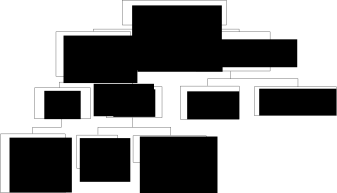
\includegraphics[width=\columnwidth, angle=-0]{hierarchy}
\caption{Hierarchy of planning approaches. See 'Handbook of Robotics, Part A: Robotic Foundations - Motion Planning' \cite{SicilianoKhatib2016} for more details.}
\end{figure}

\subsubsection{Smoothing}
One way of incorporating differential constraints into the lattice planning approach is to fit a smooth curve which respects the constraints such as a cubic spline as closely as possible to use nodes returned by the planner. The difficulty here is that the smooth curve does not exactly follow the edges in the graph which were used to calculate the route cost and check for obstacle intersection. If the cost of the smooth path is different to that of the approximation used in the lattice, any optimality guarantees provided by the planning method such as Dikstras algorithm are compromised. Worse, the smooth path must be checked against the obstacle map for collisions, and it is not clear how the path should best be modified if any collisions are detected. For an example of smoothing with clothoid curves see \cite{Lundberg2017} \cite{Walton2005}.

\subsubsection{Differential Constraints}
It is possible to carefully construct a lattice which captures differential constraints as detailed by Pivtoraiko et al \cite{Pivtoraiko2009}.The trick is calculating the control inputs required to join a set of vertices which span state space (inverse kinematics) or sampling from the control space in order to generate a set of vertices (forward kinematics). Both methods have complications, for example the shape of the lattice must be known ahead of time to be reachable with a simple set of primitives for the inverse method. For the forward method the difficulty is in the choice of interval in control space that leads to complete and uniform coverage of state space. These difficulties are resolved for one example configuration in \cite{Pivtoraiko2009} with 16 discrete headings, 8 levels of curvature and a total of 192 controls. The balance to be struck in the choice of resolution is that higher resolutions lead to a higher branching factor, increasing the memory required to represent a given area, but lower resolutions will give suboptimal paths. Imagine following a straight wall which does not align with one of the 16 cardinal directions in the lattice, but halfway between. The planner with return an optimal path which alternates between the two closest cardinal directions, rather than a straight line aligned with the wall. With a back of the envelope calculation, increasing the resolution to 10mrad to minimize artefacts increases the number of nodes required per square metre to exceed the number of atoms in the known universe. This trade off is the biggest obstacle to the use of lattice planners for general path planners and led to the development of randomized planners, which can give satisfactory uniformity and coverage of high dimensional state space without the direct link between the branching factor and the resolution when constructing a lattice.   

\subsection{Probabilistic Roadmaps}
Probabilistic Roadmaps are an example of a multiple-query sampling based planner. They are probabilistic in the sense they sample randomly from $\mathbf{W}$ to build up a connectivity graph - the roadmap. They do not inherently cope with uncertainty in the obstacle field.
One important component is a local planner, which is able to generate a path between two nearby configurations and test if it intersects with any obstacles. The algorithm proceeds by testing each sample by creating a local path from the nearest point on the existing tree, and only adding the new point to the graph is the path is obstacle free. Depending on the local planner it is possible to incorporate smooth paths respecting vehicle dynamic limits, but other methods are more appropriate in cases where the obstacle field is dynamic because the simplifying assumption making roadmaps so fast is that of a static environment. 
Another important component is the graph method used to select the shortest path such as Dijkstra which is used to find the shortest path once the roadmap is constructed. There also must be some heuristic guiding the selection of new points.

The distinction between PRMs and lattice planners is only in the mechanism by which samples are drawn from state space to construct the roadmap \cite{SicilianoKhatib2016}. They are both Roadmap planners. Either a repeating pattern or lattice is overlaid or states are selected randomly within an area of interest and discarded if they are not reachable according to the obstacle map and the local planner. This is based on the idea that randiom samples of high enough density will provide unbiased and complete coverage of the space. Particularly in the limit as the number of samples tends to infinity, a PRM may be 'probabilistically complete' so that as the number of samples tends to infinity the probability of finding a solution if one exists tends to one.

The modifications to both types of Roadmap planners which deal with a changing environment and differential constraints on motion are very similar. Differential constraints can be incorporated into the local planner as described in \ref{sec:state_lattice_planners}, alththough there are fewer constraints on PRM as there is no need to use kinmatics to ensure the samples form a regular lattice. 

\subsubsection{Uncertainty}
Both types of roadmap planner are useful for dealing with uncertain representations of the world where the environment is represented as an occupancy grid, a grid of values covering the space, each value representing the occupancy probability of that cell. The best path can be found directly from this representation by minimising the sum of occupancy probability of every cell traversed by the path. This may be more useful than the 'hard constraints' offered by optimization methods, because although the solution will not violate the constraints, the constraints themselves are constructed by throwing away information about the uncertainty of the environment to create a binary representation where every position in space is either inside or outside polygonal obstacles \cite{Pivtoraiko2009}.     

\subsection{Rapidly Exploring  Random Trees}
Rapidly Exploring Random Trees are an example of a single query planner introduced by LaValle and Kuffner \cite{LaValle2000}. Most simply, a tree is constructed by sampling from state space close to an existing node in the tree. A local planner is used to generate a trajectory from the existing node to the new sample avoiding obstacle regions if one exists. If an obstacle free trajectory is found, a new node is added at the sample state with an edge from the existing node. Nearby nodes in the tree should also be checked and connected with edges if possible. 

Starting with the initial position and the goal position, this process is repeated until sufficient coverage of the state space is obtained. When a new sample is reachable from both trees, origin and destination must be connected and a graph method such as Dijkstra can be used to identify the vertices through the graph which make up the shortest path between them. The tree growing phase of the algorithm can be terminated at this point but it may be possible to improve the quality of the solution by adding more reachable states to the connected graph in case  a better solution can be found.  

\section{Automated Intersection Management Literature Review} 
Studies on the theoretical capacity of signalized intersections and roundabouts with an equivalent footprint indicate that in most cases, if there are few approach lanes small roundabouts will tend to have higher capacity. If there are many approach lanes signals tend to be more effective, unless the traffic on different approaches is extremely unequal \cite{Jian-an2001}. 

A systematic procedure computing the conflict points in an intersection is given in \cite{Lu2013}. Roundabouts tend to have a large number of merging and diverging conflicts, but fewer or none of the crossing and head-on conflicts which lead to the most serious collisions due to high relative speeds.

Intersection control often addresses crossing conflicts by separating vehicles in time, while they all take the shortest path straight through the intersection in the same way as if it was signal controlled. There are a wide range of optimal and heuristic approaches to solve for the speed profile, both decentralized and centralized, a good review is given in \cite{Rios-Torres2017}. Many studies have looked at how to incorporate a proportion of human controlled vehicles which are not able to communicate their intention. One way of doing this is using traffic signals which only apply to human drivers \cite{Zhao2019}. The downside is that the nature of the intersection must remain similar to a traffic-light controlled one if non-communicating participants are going to be controlled by lights.

Recently a number of studies have extended intersection coordination of Connected and Autonomous Vehicles (CAVs) to the resolve the type of merging of diverging conflicts which occur and roundabouts. These are reviewed in \cite{Rios-Torres2017}. A centralized solution with an intersection manager minimizing delay and energy consumption is described in \cite{Zhao2018}. This shows that a high proportion of vehicles need to be communicating for significant benefits to be realized. 

A decentralized approach based on intent communication by way of virtual vehicles, can also be applied to roundabouts. In \cite{Debada2016}, reactive heuristics are shown to lead to poor performance compared to a model predictive control approach. The virtual vehicle concept allows common lane based heuristics such as car following to be extended to resolve conflicts in  \cite{Debada2018}. Another work investigating virtual lanes is \cite{Xu2018}. Here a conflict graph is used to assign approaching vehicles to appropriate virtual lanes and a distributed controller is presented to stabilize the platoon.

Another approach presented in \cite{Liu2018} is a decentralized solution to the global problem of minimizing the delay. Proofs of completeness and optimality of the aggregate problem are given, making this technique very impressive. It is not shown to be applicable to roundabouts in any of the numerical examples, although the incorporation of optimal trajectory planning by the low level controller to execute merging makes it a good example of the combination of path planning and intersection management. Collision constraints are based on a conflict zone rather than conflict points as in \cite{Levin2017}. The location of the conflict points is fixed by the fixed paths between the entry and exit lanes of the junction. The space inefficiency of the zone representation for multiple lanes is addressed by using multiple zones, one for each pair of lanes. The use of simultaneous path optimization might be expected to increase computational complexity and thereby reduce the number of vehicles with can be routed, however an attached video showing many vehicles interacting for about 10 minutes seems to refute this. It seem the ordering problem is resolved in a decentralized way based on game theory and the game `Chicken.' Using game theory to resolve the ordering problem may give this approach an edge over the mixed integer optimization used in \cite{Levin2017}, in terms of how many vehicles they can control before running into execution time limits. It is a little surprising that the game would always produce the optimal ordering given the motion model used by each AGV. The consensus mechanism will be important here. Questions remain about the possibility of AGVs disagreeing about the order they calculate from the communicated position and speed data. 

A similar method which solves the ordering ordering problem sequentially, followed by individual optimization of the approach speed along fixed paths is described in \cite{DeCampos2017}. This method claims only local (per-vehicle) optimality for the speed choice sub problem, and makes it clear the crossing order at convergence will be suboptimal, and depends strongly on the decision order. The sub problem is posed as a Linear Quadratic Regulator, commonly seen in optimal control problems. In general terms, those early in the decision order will deviate from the plans less. This is more of a problem when vehicles are not uniform, as to reduce energy consumption a late arriving lorry should deviate as little as possible. A heuristic is given for the decision order based on the time to conflict arrival.

The use of optimal control in \cite{DeCampos2017} is shared with many earlier works regarding coordination of Unmanned Arial Vehicles, many of which relax the assumption of static paths. In this way \cite{Schouwenaars2004} addressed the full multi-vehicle motion planning problem for small numbers of aircraft with simple dynamics. The craft were assumed to be differentially flat: that is, able to actuate in any of the workspace degrees of freedom independently, like a quadrotor. They were represented using bounding rectangles, leading to a slightly conservative mixed integer problem. The integer variables are used to choose which constraints are active. This might seem excessive when representing static obstacles, however when the constraints arise from other moving vehicles, the integer variables are a natural way to represent the passing-order problem. The scaling to larger numbers of vehicles is a particular challenge, due to the combinatorial explosion of possibilities.

An alternative approach to the coordination of differentially flat aircraft which uses a sequential solution of per-vehicle receding horizon sub problems to approximate the global solution is given in \cite{Keviczky2008}. An earlier theoretical treatment based on iterative bargaining with soft collision constraints is given by \cite{Inalhan2002}. The parameters are real numbers, and the constraints linear while the cost is quadratic. It may converge to an infeasible solution given a particular minimum safety distance even from a valid set of starting positions and speeds, and the suggested solution is to reduce the threshold until it becomes feasible.  

More recently, solutions based on Distributed Model Predictive (DMPC) control have been developed. In \cite{Dai2017}, per-vehicle optimizations runs simultaneously to reduce execution time. This ensures recursive feasibility and closed loop stability. Another DMPC approach is given by \cite{Luis2018}. This scales up to 25 vehicles in real time. the quadrotors concerned are all identical and differentially flat. For an under-actuated system like an AGV, some of the simplifications may no longer be possible.
